\chapter{Opis problema}
\label{ch:opis-problema}
Ovaj rad bavi se problemom raspoznavanja studentskih identifikacijskih brojeva, poznatih pod skraćenicom
\emph{JMBAG}\footnote{\emph{Jedinstveni Matični Broj Akademskog Građana.}}. Ti se brojevi sastoje od deset znamenaka i
svakom studentu je dodijeljen jedinstveni broj koji služi kao identifikator studenta u sustavu hrvatskih fakulteta.
Kod pristupanja ispitima, od studenata se očekuje da uz ime i prezime također napišu svoj \emph{JMBAG} kako bi ih se
moglo jedinstveno identificirati u sustavu. Stoga je korisno napraviti sustav koji će moći automatski raspoznavati te
brojeve. Problem raspoznavanja \emph{JMBAG}-ova može se podijeliti u tri faze: pretprocesiranje, segmentacija i
klasifikacija. Faza pretprocesiranja služi kako bi se ulazna slika normalizirala te kako bi se znamenke odvojile od
pozadine. U fazi segmentacije potrebno je odrediti granice između pojedinačnih znamenki \emph{JMBAG}-a kako bi se svaka
znamenka mogla pojedinačno raspoznavati. Moguće je raspoznavati i više znamenki odjednom, ali tada klasifikator mora
biti kompleksniji i skup podataka za učenje mora biti veći. Zbog toga je poželjnije raspoznavati pojedinačne znamenke,
jer se skup za učenje efektivno poveća deset puta i sam klasifikator može biti jednostavniji. Posljednja faza
klasifikacije raspoznaje svaku znamenku pojedinačno. Slijednim spajanjem pojedinačno klasificiranih brojeva dobiva se
konačno raspoznati \emph{JMBAG}. U sljedećim odjeljcima bit će opisana implementacija navedenih faza raspoznavanja te
njihovo povezivanje u sustav za raspoznavanje \emph{JMBAG}-ova. Također će biti opisan postupak učenja i treniranja
unaprijedne neuronske mreže koja je korištena kao klasifikator pojedinačnih znamenaka \emph{JMBAG}-a.


\section{Pretprocesiranje}
\label{sec:pretprocesiranje}
\begin{figure}[htb]
    \centering
    
\includegraphics[width=12cm]{images/preprocessing-original-image.png}
    \caption{\emph{JMBAG} prije pretprocesiranja.}
    \label{fig:preprocessing-original-image}
\end{figure}
Faza pretprocesiranja omogućuje jednoliko tretiranje ulaznih slika u preostalim fazama raspoznavanja. To se postiže na
način da se ulazna slika binarizira - dio slike koji predstavlja broj mora biti jasno odvojen od pozadine slike. Nakon
učitavanja slike u memoriju, prvi korak prema binarizaciji je uklanjanje svih boja iz slike. Time će se dobiti slika u
nijansama sive boje nad kojom se dalje može provesti postupak binarizacije. Kako bi se uklonila boja iz slike, za svaki
piksel računa se njegov intenzitet na sljedeći način:\\
\begin{equation*}
    I = \left(\frac{I_{crvena} + I_{zelena} + I_{plava}}{765}\right)^{2} \cdot 255.
\end{equation*}\\
Kako se piksel sastoji od komponenata $I_{crvena}$, $I_{zelena}$ i $I_{plava}$ čiji je raspon vrijednosti $[0, 255]$,
pri izračunu intenziteta njihov zbroj dijelimo sa zbrojem njihovih maksimalnih vrijednosti ($3 \cdot 255 = 765$).
Dobiveni rezultat zatim kvadriramo kako bi se bolje aproksimirala percepcija ljudskog oka na svjetlinu. Na kraju,
kvadrirani rezultat pomnoži se s $255$ kako bi se opet dobila vrijednost u rasponu $[0, 255]$. Dobiveni intenzitet $I$
zatim se koristi kao nova vrijednost komponenata $I_{crvena}$, $I_{zelena}$ i $I_{plava}$ za taj piksel.\\
\begin{figure}[htb]
    \centering
    
\includegraphics[width=12cm]{images/preprocessing-grayscale-image.png}
    \caption{\emph{JMBAG} nakon uklanjanja boje iz slike.}
    \label{fig:preprocessing-grayscale-image}
\end{figure}
Sada kada je za svaki piksel izračunat njegov intenzitet, može se provesti postupak binarizacije. Prvo je potrebno
pronaći minimalnu vrijednost intenziteta $I_{\min}$ i maksimalnu vrijednost intenziteta $I_{\max}$ na cijeloj slici za
sve potpuno vidljive piksele\footnote{Piksel se smatra potpuno vidljivim ako je vrijednost njegove neprozirnosti
jednaka $255$.}. Preko $I_{\min}$ i $I_{\max}$ računa se intenzitet odsijecanja:\\
\begin{equation*}
    I_{o} = I_{\max} - I_{\min}.
\end{equation*}\\
Intenzitet odsijecanja $I_{o}$ zatim se koristi kako bi se slika binarizirala na sljedeći način:
\begin{enumerate}
    \item Ako je vrijednost neprozirnosti piksela $(x, y)$ manja od $255$, piksel će pripadati pozadini.
    \item Ako je intenzitet piksela $(x, y)$ veći od intenziteta odsijecanja $I_{o}$, piksel će pripadati pozadini.
    \item Inače će piksel pripadati \emph{JMBAG}-u koji se raspoznaje.
\end{enumerate}
Kod binarizacije su pikseli pozadine bijele boje, dok su pikseli \emph{JMBAG}-a crne boje.
Slike\ \ref{fig:preprocessing-original-image},\ \ref{fig:preprocessing-grayscale-image}
i\ \ref{fig:preprocessing-binarized-image} prikazuju jedan \emph{JMBAG} kroz opisane korake pretprocesiranja.
\begin{figure}[htb]
    \centering
    
\includegraphics[width=12cm]{images/preprocessing-binarized-image.png}
    \caption{\emph{JMBAG} nakon postupka binarizacije.}
    \label{fig:preprocessing-binarized-image}
\end{figure}


\section{Segmentacija}
\label{sec:segmentacija}
Nakon binarizacije potrebno je pronaći granice među brojevima \emph{JMBAG}-a kako bi se oni mogli zasebno raspoznavati
u klasifikatoru. Kako slika dobivena postupkom binarizacije sadrži samo crnu i bijelu boju, za postupak segmentacije
korištena je pretpostavka da su brojevi na slici pojedinačno odvojene komponente. Stoga prvi korak segmentacije
pronalazi sve crne povezane komponente na slici te ih grupira u međusobno disjunktne skupove piksela koje će se u
daljnjem tekstu nazivati grupama piksela. U idealnom slučaju, svaka znamenka sastojat će se od samo jedne grupe piksela
koja je odvojena od svih ostalih grupa znamenaka, time ukupno tvoreći 10 grupa piksela. Ovakav slučaj prikazan je na
slici\ \ref{fig:ideal-segmentation} gdje je svaka grupa piksela obojana različitom bojom.
\begin{figure}[htb]
    \centering
    
\includegraphics[width=12cm]{images/ideal-segmentation.png}
    \caption{Idealno odvojene znamenke \emph{JMBAG}-a.}
    \label{fig:ideal-segmentation}
\end{figure}
Međutim, ovo neće uvijek biti slučaj te će neke slike sadržavati veći ili manji broj grupa piksela koje ne moraju nužno
odgovarati pojedinačnim znamenkama. Kako bi se za takve slike proveo postupak segmentacije, pronađene grupe piksela
dijele se na glavne grupe piksela i sporedne grupe piksela. Glavne grupe piksela čini skupina od najviše 10 grupa
piksela sa slike koje pojedinačno sadrže barem $\frac{1}{30}$ ukupnog broja crnih piksela na slici, dok su sve ostale
grupe sporedne grupe. Time je osigurano da će glavnih grupa uvijek biti 10 ili manje. Ovisno o broju pronađenih glavnih
grupa, implementirani algoritam segmentacije podešava skup glavnih grupa na sljedeći način:
\begin{enumerate}
    \item Ako je pronađeno 10 glavnih grupa, skup glavnih grupa ne treba podešavati.
    \item Ako je pronađeno 9 glavnih grupa, glavna grupa najveće širine uklanja se iz skupa glavnih grupa te se dijeli
    na pola po širini. Time se dobivaju dvije nove grupoe piksela koje se dodaju u skup glavnih grupa koji tada sadrži
    ukupno 10 grupa.
    \item Ako je pronađeno 8 glavnih grupa, dvije glavne grupe najveće širine uklanjaju se iz skupa glavnih grupa.
    Zatim se uspoređuje omjer širina najšire i druge najšire uklonjene grupe. Ako je taj omjer veći ili jednak $1.33$,
    najšira grupa dijeli se na tri jednaka dijela po širini te se tako dobivene grupe zajedno s preostalom grupom dodaju
    u skup glavnih grupa. S druge strane ako je omjer širina manji od $1.33$, obje uklonjene grupe dijele se na pola po
    širini te se novonastale grupe dodaju u skup glavnih grupa. U oba slučaja, skup glavnih grupa sadržavat će ukupno 10
    grupa.
    \item Ako je pronađeno 7 ili manje glavnih grupa, tada se $10 - n$ najširih grupa dijeli na pola po širini, gdje je
    $n$ broj pronađenih glavnih grupa.
\end{enumerate}
Ako nakon prethodnog koraka podešavanja skup glavnih grupa ne sadrži ukupno 10 grupa, algoritam segmentacije označava
sliku kao neispravnu te se postupak klasifikacije neće provoditi za tu sliku. U suprotnom, algoritam nastavlja s radom.
Slike\ \ref{fig:segmentation-before-division} i\ \ref{fig:segmentation-after-division} prikazuju navedeni proces
podešavanja glavnih grupa za slučaj 9 pronađenih glavnih grupa. Slika\ \ref{fig:segmentation-before-division} prikazuje
stanje prije podešavanja glavnih grupa te je na njoj najšira grupa označena sivom bojom, dok
slika\ \ref{fig:segmentation-after-division} prikazuje konačnu podjelu glavnih grupa nakon podešavanja.\\
\begin{figure}[htb]
    \centering
    
\includegraphics[width=12cm]{images/segmentation-before-division.png}
    \caption{\emph{JMBAG} s dvije povezane znamenke prije podešavanja glavnih grupa piksela.}
    \label{fig:segmentation-before-division}
\end{figure}
\begin{figure}[htb]
    \centering
    
\includegraphics[width=12cm]{images/segmentation-after-division.png}
    \caption{\emph{JMBAG} s dvije povezane znamenke nakon podešavanja glavnih grupa piksela.}
    \label{fig:segmentation-after-division}
\end{figure}
Sljedeći korak jest pronaći kojim glavnim grupama teže pojedinačne sporedne grupe. Prvo se za svaku grupu računa
središte $(x_s, y_s)$:\\
\begin{align*}
    x_s = \frac{\sum_{n = 1}^{N} x_n}{N}\\
    y_s = \frac{\sum_{n = 1}^{N} y_n}{N}
\end{align*}\\
gjde je $N$ broj crnih piksela u grupi. Za svako središte glavne grupe $(x_{s_g}, y_{s_g})$ i središte sporedne grupe
$(x_{s_s}, y_{s_s})$ računa se njihova međusobna \emph{Euklidska} udaljenost:\\
\begin{equation*}
    D = \sqrt{(x_{s_g} - x_{s_s})^{2} + (y_{s_g} - y_{s_s})^{2}}
\end{equation*}\\
te se svaka sporedna grupa pridjeljuje najbližoj glavnoj grupi. Nakon opisanog posupka postojati će 10 grupa piksela
na temelju kojih se svaka znamenka izdvaja u zasebnu sliku. Slika\ \ref{fig:unassigned-minor-groups} prikazuje stanje
prije dodjeljivanja sporednih grupa (označenih crnom bojom) glavnim grupama, dok slika\ \ref{fig:assigned-minor-groups}
prikazuje stanje nakon dodjeljivanja.
\begin{figure}[htb]
    \centering
    
\includegraphics[width=12cm]{images/unassigned-minor-groups.png}
    \caption{Glavne i sporedne grupe piksela prije postupka dodjeljivanja.}
    \label{fig:unassigned-minor-groups}
\end{figure}
\begin{figure}[htb]
    \centering
    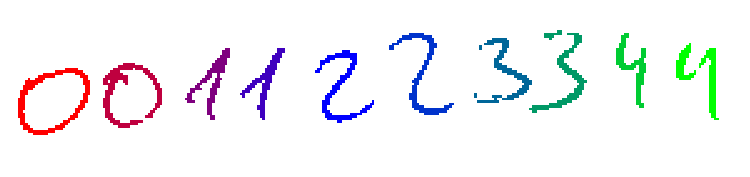
\includegraphics[width=12cm]{images/assigned-minor-groups.png}
    \caption{Glavne i sporedne grupe piksela nakon postupka dodjeljivanja.}
    \label{fig:assigned-minor-groups}
\end{figure}


\section{Klasifikacija}
\label{sec:klasifikacija}


\section{Postupak učenja neuronske mreže}
\label{sec:postupak-ucenja-neuronske-mreze}
